%%%%%%%%%%%%%%%%%%%%%%%%%%%%%%%%%%%%%%%%%
%
% CMPT xxx
% Some Semester
% Lab/Assignment/Project X
%
%%%%%%%%%%%%%%%%%%%%%%%%%%%%%%%%%%%%%%%%%

%%%%%%%%%%%%%%%%%%%%%%%%%%%%%%%%%%%%%%%%%
% Short Sectioned Assignment
% LaTeX Template
% Version 1.0 (5/5/12)
%
% This template has been downloaded from: http://www.LaTeXTemplates.com
% Original author: % Frits Wenneker (http://www.howtotex.com)
% License: CC BY-NC-SA 3.0 (http://creativecommons.org/licenses/by-nc-sa/3.0/)
% Modified by Alan G. Labouseur  - alan@labouseur.com
%
%%%%%%%%%%%%%%%%%%%%%%%%%%%%%%%%%%%%%%%%%

%----------------------------------------------------------------------------------------
%	PACKAGES AND OTHER DOCUMENT CONFIGURATIONS
%----------------------------------------------------------------------------------------

\documentclass[letterpaper, 10pt,DIV=13]{scrartcl} 

\usepackage[T1]{fontenc} % Use 8-bit encoding that has 256 glyphs
\usepackage[english]{babel} % English language/hyphenation
\usepackage{amsmath,amsfonts,amsthm,xfrac} % Math packages
\usepackage{sectsty} % Allows customizing section commands
\usepackage{graphicx}
\usepackage[lined,linesnumbered,commentsnumbered]{algorithm2e}
\usepackage{listings}
\usepackage{parskip}
\usepackage{lastpage}

\allsectionsfont{\normalfont\scshape} % Make all section titles in default font and small caps.

\usepackage{fancyhdr} % Custom headers and footers
\pagestyle{fancyplain} % Makes all pages in the document conform to the custom headers and footers

\fancyhead{} % No page header - if you want one, create it in the same way as the footers below
\fancyfoot[L]{} % Empty left footer
\fancyfoot[C]{} % Empty center footer
\fancyfoot[R]{page \thepage\ of \pageref{LastPage}} % Page numbering for right footer

\renewcommand{\headrulewidth}{0pt} % Remove header underlines
\renewcommand{\footrulewidth}{0pt} % Remove footer underlines
\setlength{\headheight}{13.6pt} % Customize the height of the header

\numberwithin{equation}{section} % Number equations within sections (i.e. 1.1, 1.2, 2.1, 2.2 instead of 1, 2, 3, 4)
\numberwithin{figure}{section} % Number figures within sections (i.e. 1.1, 1.2, 2.1, 2.2 instead of 1, 2, 3, 4)
\numberwithin{table}{section} % Number tables within sections (i.e. 1.1, 1.2, 2.1, 2.2 instead of 1, 2, 3, 4)

\setlength\parindent{0pt} % Removes all indentation from paragraphs.

\binoppenalty=3000
\relpenalty=3000

%----------------------------------------------------------------------------------------
%	TITLE SECTION
%----------------------------------------------------------------------------------------

\newcommand{\horrule}[1]{\rule{\linewidth}{#1}} % Create horizontal rule command with 1 argument of height

\title{	
   \normalfont \normalsize 
   \textsc{CMPT 424 - Fall 2023 - Dr. Labouseur} \\[10pt] % Header stuff.
   \horrule{0.5pt} \\[0.25cm] 	% Top horizontal rule
   \huge Lab 5  \\     	    % Assignment title
   \horrule{0.5pt} \\[0.25cm] 	% Bottom horizontal rule
}

\author{Luciano Mattoli \\ \normalsize luciano.mattoli1@Marist.edu}

\date{\normalsize\today} 	% Today's date.

\begin{document}
\maketitle % Print the title

%----------------------------------------------------------------------------------------
%   start QUESTIONS
%----------------------------------------------------------------------------------------
\section{Questions}

\subsection{Consider the following set of processes, with the length of the CPU burst given in milliseconds:}

\begin{table}
    \centering
    \begin{tabular}{ccc}
         Process&  Burst Time& Priority\\
         P1&  10& 3\\
         P2&  1& 1\\
         P3&  2& 3\\
         P4&  1& 4\\
         P5&  5& 2\\
    \end{tabular}
    \caption{Table}
    \label{tab:my_label}
\end{table}
The processes are assumed to have arrived in the order P1, P2, P3, P4, P5, all at time 0.

\begin{itemize}
    \item Draw four Gantt charts that illustrates the execution of these processes using the followings scheduling algorithms: FCFS, SJF, nonpreemptive priority (a smaller priority number implies a higher priority), and RR (quantum = 1).
\begin{figure}
    \centering
    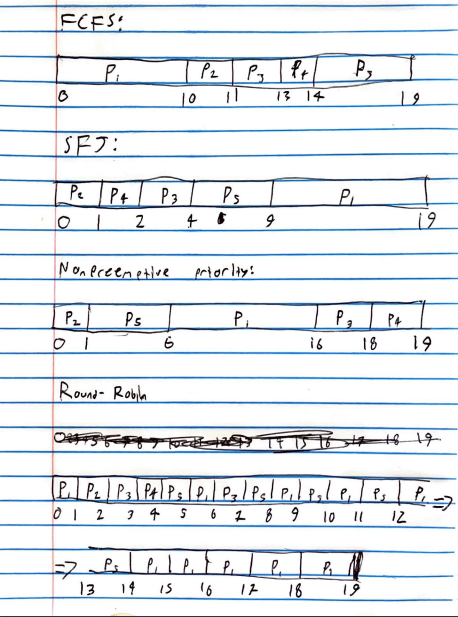
\includegraphics[width=0.75\linewidth]{lab5.png}
    \caption{Gantt charts for FCFS, SJF, nonpreemptive priority, and round-robin}
    \label{fig:enter-label}
\end{figure}
    \item What is the turnaround time of each process for each of the scheduling algorithms in part a?
    \begin{itemize}
        \item FCFS: P1 = 10ms, P2 = 11ms, P3 = 13ms, P4 = 14ms, P5 = 19ms
        \item SJF: P1 = 19ms, P2 = 1ms, P3 = 4ms, P4 = 2ms, P5 = 9ms
        \item Nonpreemptive Priority: P1 = 16ms, P2 = 1ms, P3 = 18ms, P4 = 19ms, P5 = 6ms
        \item Round-Robin: P1 = 19ms, P2 = 2ms, P3 = 7ms, P4 = 4ms, P5 = 14ms
    \end{itemize}
    \item What is the waiting time of each process for each of these scheduling algorithms?
    \begin{itemize}
        \item FCFS: P1 = 0ms, P2 = 10ms, P3 = 11ms, P4 = 13ms, P5 = 14ms
        \item SJF: P1 = 9ms, P2 = 0ms, P3 = 2ms, P4 = 1ms, P5 = 4ms
        \item Nonpreemptive Priority: P1 = 6ms, P2 = 0ms, P3 = 16ms, P4 = 18ms, P5 = 1ms
        \item Round-Robin: P1 = 9ms, P2 = 1ms, P3 = 5ms, P4 = 3ms, P5 = 9ms
    \end{itemize}
    \item Which of the algorithms results in the minimum average waiting time (over all processes)?
    \begin{itemize}
        \item FCFS = 9.6ms
        \item SJF = 3.2ms
        \item Nonpreemptive Priority = 8.2ms
        \item Round-Robin = 5.4ms
Shortest-Job-First Scheduling results in the minimum average waiting time with 3.2ms.
    \end{itemize}
\end{itemize}

%----------------------------------------------------------------------------------------
%   end QUESTIONS
%----------------------------------------------------------------------------------------

\pagebreak

\end{document}
